\section{Feature Extraction with Linear Features}
\label{sec:extraction}
\subsection{Overview}
One of the most ubiquitous features of any indoor environment are walls. While it maybe necessary to find other obstacles and landmarks, for path planning and mapping, knowing the locations of walls always advantageous. At the very least it can be used to remove the laser readings close to it reducing the data set to be further analyzed by methods such as clustering. In relatively clean environments, such as corridors that are not too crowded, walls will usually suffice for \slam. Also algorithms that find linear features are more robust to humans moving around in the environment than those finding cylinders or generic features in the data. Also since the feature we are trying to extract is a wall, it is reasonable to model it as a line of infinite length which reduces the dimensions of state required to represent it. Similar to section \ref{sec:Spike_math} once the walls have been detected, a measurement model is required to calculate the innovation. It is obvious that the measurement model and it's derivatives will not be the same as in point features as the wall moves very differently as the robot moves. For example, when the robot is moving parallel to the wall, the LIDAR scan from one time step to another will be identical, but unlike in the case of point features that need not imply the robot has not moved. So different measurement models are developed and their Jacobian matrices calculated for linear features. 

\subsection{RANSAC based Feature Extraction Algorithm}
\label{sec:ransac}
The fundamental concept in extracting linear features is to fit a line or multiple lines onto a set of points. There are a large number of methods to do that such as least squares, Split-merge and RANSAC\cite{Nguyen2005}. Looking into a few implementations of RANSAC in common libraries such as PCL and OpenCV, we see that it tries to robustly fit a line to a given set of points. In regular environments, since more than one wall can be seen at a time, it becomes necessary to first segment the data before using the algorithm. Instead another approach is to randomly sample points and try to fit multiple lines simultaneously. This approach is explained in algorithm \ref{alg: RANSAC algorithm}\cite{riisgaard2003slam}.

\begin{algorithm}[H]
\begin{algorithmic}

	\While{
	\begin{itemize}
		\item there are still unassociated laser readings, 
		\item and the number of readings is larger than the consensus, 
		\item and we have done less than N trials.
	\end{itemize}
	}
	\begin{itemize}
	\item Select a random laser data reading. 
	\item Randomly sample S data readings within D degrees of this laser 
	data reading 
	\item Using these S samples and the original reading calculate a 
	least squares best fit line. 
	\item Determine how many laser data readings lie within X distance 
	from this best fit line
	\item If the number of laser data readings on the line is above some 
	consensus C do the following: 
		\begin{itemize}
			\item calculate new least squares best fit line based on all 
			the laser readings determined to lie on the old best fit 
			line. 
			\item Add this best fit line to the lines we have extracted. 
			\item Remove the number of readings lying on the line from the 
			total set of unassociated readings.
		\end{itemize}
	\end{itemize}
	\EndWhile
\end{algorithmic}
	\caption{Multiple line fitting with RANSAC.}
	\label{alg: RANSAC algorithm}
\end{algorithm}

\subsection{RANSAC Examples}
 \begin{figure}[h!]
     \centering
     \begin{subfigure}[b]{0.45\textwidth}
     
 	    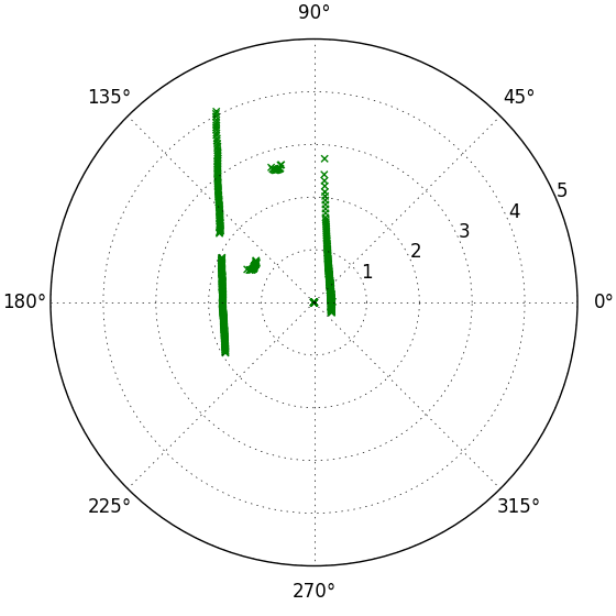
\includegraphics[width=\textwidth]{blank_scan}
         \caption{Polar plot of laser scan.}
     \end{subfigure}
     \quad %add desired spacing between images, e. g. ~, \quad, \qquad, \hfill etc.
       %(or a blank line to force the subFigure~onto a new line)
     \begin{subfigure}[b]{0.45\textwidth}
         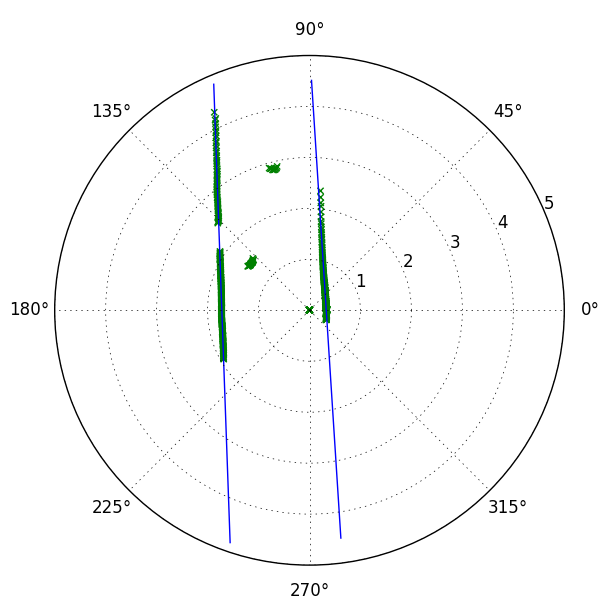
\includegraphics[width=\textwidth]{ransac_good}
		 \caption{Detected lines.}
     \end{subfigure}%
         \caption{Example of walls detected by RANSAC.}
         \label{fig: ransac_good}
 \end{figure}
 Considering the same setup as in Figure~\ref{fig:Real world arena}, we can try the RANSAC algorithm on the data collected from the LIDAR. It is seen to give good results initially as seen in Figure~\ref{fig: ransac_good}. As we move forward though the result is not always maintained. Looking at algorithm \ref{alg: RANSAC algorithm} it is possible that since the first laser reading is chosen at random, it may not be on a wall at all. S readings in it's neighborhood could generate a line that is at a small angle to both walls in the environment. Since it is close enough to the walls, a large number of points will wrongly be associated to this, which will result in a spurious wall being detected.This will have a detrimental effect in all the further time steps. An example of this is seen in Figure~\ref{fig: ransac_bad}.
 \begin{figure}[h!]
     \centering
     \begin{subfigure}[b]{0.45\textwidth}
     
 	    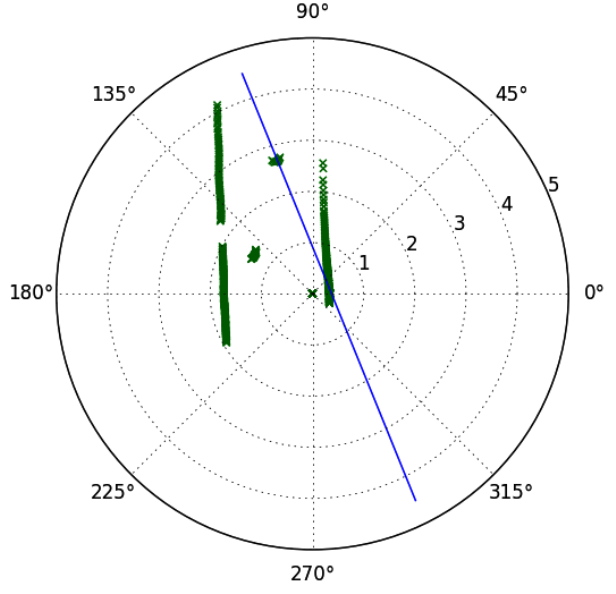
\includegraphics[width=\textwidth]{ransac_bad}
        \caption{Detected lines.}
     \end{subfigure}
     \quad %add desired spacing between images, e. g. ~, \quad, \qquad, \hfill etc.
       %(or a blank line to force the subFigure~onto a new line)
     \begin{subfigure}[b]{0.45\textwidth}
         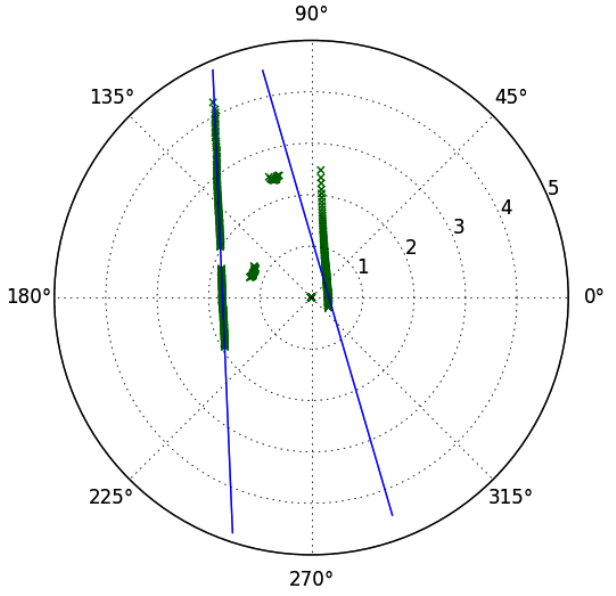
\includegraphics[width=\textwidth]{ransac_bad1}
		 \caption{Detected lines.}
     \end{subfigure}%
         \caption{Example of spurious walls marked by RANSAC.}
         \label{fig: ransac_bad}
 \end{figure}
\subsection{Hough transform based Feature Extraction Algorithm}
\label{sec:hough}
In the fields of image analysis and computer vision, hough transform is a very popular feature extraction technique\cite{Stockman2001}. While it was originally designed to find lines in an image can be used to detect any shape as long as that shape can be represented in a mathematical form\cite{Duda1972}. It can detect the shape in spite of distortions making it much more robust than RANSAC\cite{Hu1998}. In the current application the aim is to find walls in the range data of the LIDAR. Hence the first step is to rasterize the points into an image so that we can use the OpenCV implementation of Hough Transform. The image is then converted to a binary image and then passed to the hough transform function. The algorithm itself is described below.

In image processing, a common way of representing lines is the normal form of a line equation, 
\begin{equation}[h!]
r=x\cos\theta+y\sin\theta
\label{eq:hough1}
\end{equation}
In this form a line is completely defined by 2 variables $ r $ and  $ \theta $. The first step of finding lines in an image is that for any point $ (x_0,y_0) $ in the image, a family of lines passing through that point is expressed as,

\begin{equation}[h!]
r_\theta=x_0\cos\theta+y_0\sin\theta
\label{eq:hough2}
\end{equation}

Since all lines are assumed to be infinite in both directions, $ \theta $ can only take unique values between $ 0^\circ $ and $ 180^\circ $. This range is then discretized to give a fixed number of possible line angles. The range $ r $ is also discretized based on the resolution required. For single pixel resolution the possible ranges will be all numbers from 0 to the length of the diagonal of the image. Since this will result in a large number of possible $ r $ values, a lower resolution will considerably speed up the algorithm. Now that there is a fixed number for possible $ r $ and $ \theta $, a 2D matrix of zeros is created in which each row corresponds to a possible value of $ \theta $ and each column to $ r $ as in Equation~\ref{eq:hough3}. This is called the accumulator. 

\begin{equation}
A=\bordermatrix{~  & r_1 & r_2&\ldots & r_n \cr
              \theta_1& 0 &  0  & \ldots & 0\cr
              \theta_2& 0  &  0 & \ldots & \cr
              \vdots& \vdots & \vdots & \ddots & \vdots\cr
              \theta_n& 0  &   0       &\ldots & 0}
\label{eq:hough3}
\end{equation} 

 Once this initial setup is complete, a non zero point on the binary image $ (x_0,y_0) $ is chosen at random. For this point the family of lines passing through it will be given by Equation~\ref{eq:hough2}. For each possible $ \theta $ the corresponding $ r $ is calculated from the same equation. For each $ (r,\theta) $ pair found, the corresponding entry in the accumulator $ A $ is incremented. Once all the possible pairs are calculated, a different image point is chosen till all the non zero points on the image are explored. 
 
 The accumulator now represents all possible lines in the image and the number of points that lie on each of the lines. The accumulator entries that are greater than a certain preset threshold represent the lines in the image. The $ (r,\theta) $ values corresponding to these lines are returned. 
 
 An important aspect of using the Hough transform from OpenCV is the conversion of LIDAR data to image and the detected lines back to the robot frame of reference. The former is straight forward. Since the range of the LIDAR is known, the image size can be fixed based on the resolution required. For, example the LIDAR described in chapter \ref{cha:Platform} has a maximum range of $ 5 m $. So for a resolution of $ 1 cm $, a blank image of $ 500 \times 500 $ pixels is created. When each LIDAR point is converted to Cartesian coordinates $ (x_l,y_l) $, they are with respect to an origin at the LIDAR itself. OpenCV images on the other hand, follow a coordinate system that has the origin in the top right corner of the image. Hence each point is mapped to the image coordinate frame using a homogeneous transformation,
 \begin{equation}
 \begin{bmatrix}
 x_i\\y_i\\1
 \end{bmatrix}=
 \begin{bmatrix}
 0 & -1 & 500\\
 1 & 0 & 500\\
 0 & 0 & 1
 \end{bmatrix}
 \begin{bmatrix}
 x_l\\y_l\\1
 \end{bmatrix}
 \label{eq:hough4}
 \end{equation}
 
The image points are then rounded to the nearest centimeter and the pixel corresponding to that value is set to white. This gives an image with black background and all the Laser readings shown in white which can be passed to the hough transform function. It may sometimes be required to erode and dilate the image with different kernels to make the points more visible. 
 
The lines returned by the hough transform, are in units of pixels and are with reference the image origin. To convert it to the robot frame, 2 points are chosen on the line and each of these points are mapped to the robot frame using the inverse transformation of Equation~\ref{eq:hough4} and the normal form of the Equation~of the line passing through these 2 points is found. 

\subsection{Hough Transform Examples}
In the same arena as in Figure~\ref{fig:Real world arena}, the hough transform is found to be really robust in finding the walls as seen in Figure~\ref{fig: hough1}.
 \begin{figure}[h!]
     \centering
     \begin{subfigure}[b]{0.45\textwidth}
     
 	    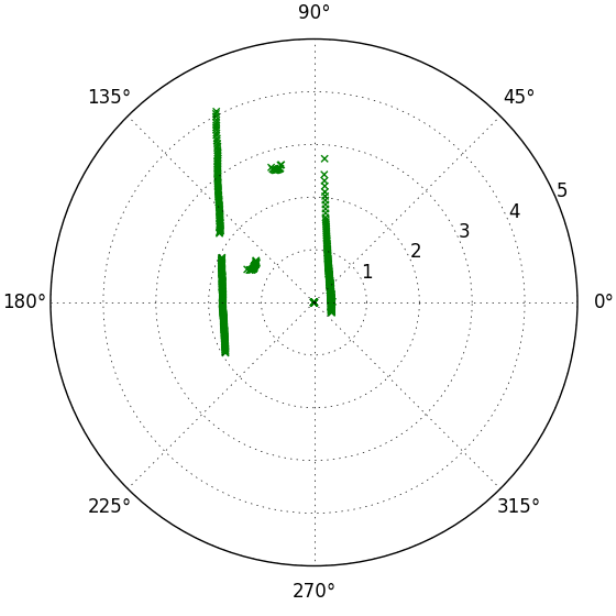
\includegraphics[width=\textwidth]{blank_scan}
         \caption{Polar plot of laser scan.}
     \end{subfigure}
     \quad %add desired spacing between images, e. g. ~, \quad, \qquad, \hfill etc.
       %(or a blank line to force the subFigure~onto a new line)
     \begin{subfigure}[b]{0.45\textwidth}
         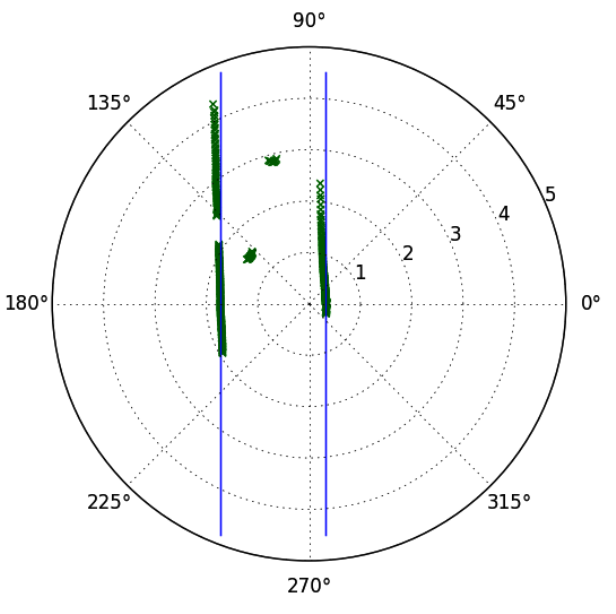
\includegraphics[width=\textwidth]{hough1}
		 \caption{Detected lines.}
     \end{subfigure}%
         \caption{Example of walls detected by Hough Transform.}
         \label{fig: hough1}
 \end{figure}

Unlike the RANSAC algorithm, the hough transform considers all possible lines before deciding on any line, it is robust to noise in the surroundings. This is especially useful when there are people walking around in the environment.
 \begin{figure}[h!]
     \centering
     \begin{subfigure}[b]{0.45\textwidth}
     
 	    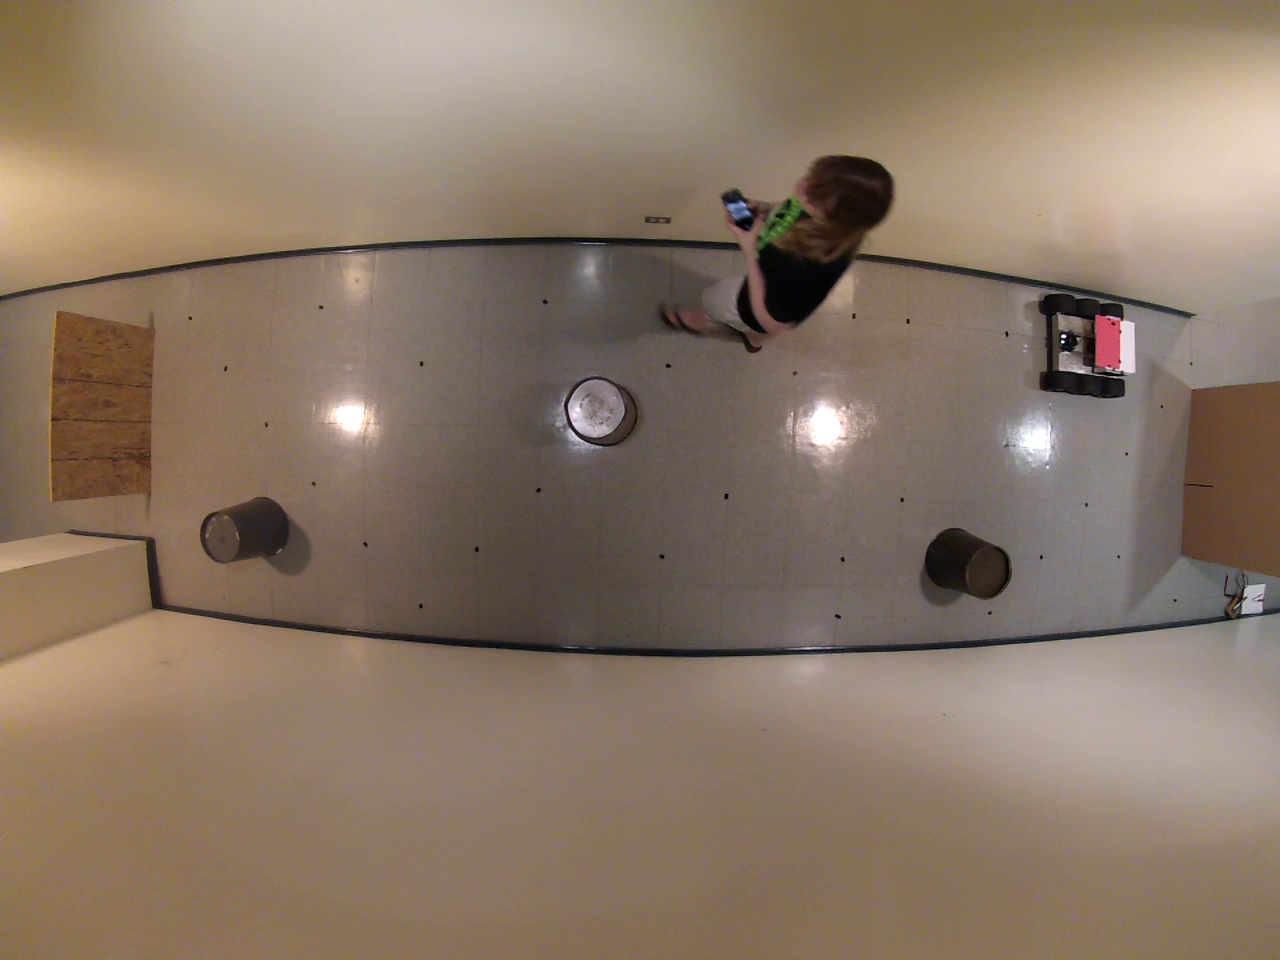
\includegraphics[width=\textwidth]{overhead2}
         \caption{Overhead view of the arena.}
     \end{subfigure}
     \quad %add desired spacing between images, e. g. ~, \quad, \qquad, \hfill etc.
       %(or a blank line to force the subFigure~onto a new line)
     \begin{subfigure}[b]{0.45\textwidth}
         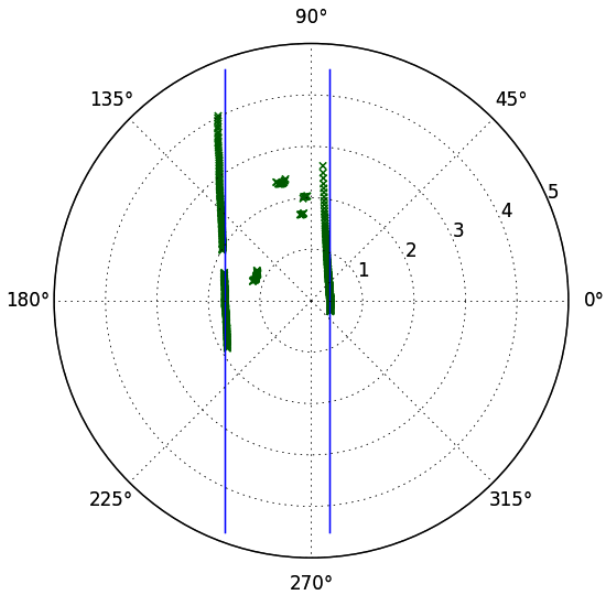
\includegraphics[width=\textwidth]{hough2}
		 \caption{Detected lines}
     \end{subfigure}%
         \caption{Example 1 of Hough Transform being robust to people.}
         \label{fig: hough2}
 \end{figure}
 
  \begin{figure}[h!]
      \centering
      \begin{subfigure}[b]{0.45\textwidth}
      
  	    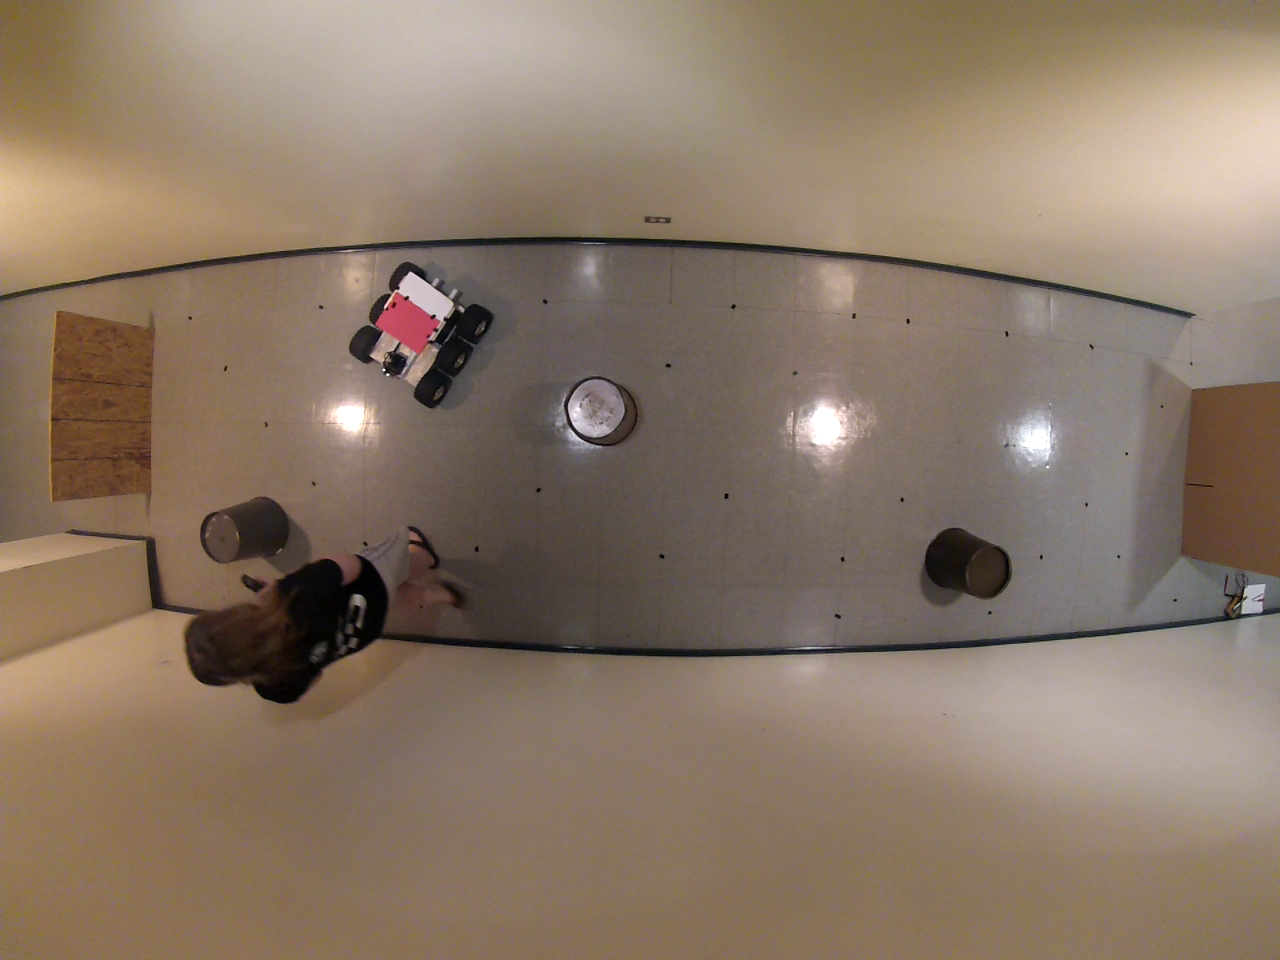
\includegraphics[width=\textwidth]{overhead3}
          \caption{Overhead view of the arena}
      \end{subfigure}
      \quad %add desired spacing between images, e. g. ~, \quad, \qquad, \hfill etc.
        %(or a blank line to force the subFigure~onto a new line)
      \begin{subfigure}[b]{0.45\textwidth}
          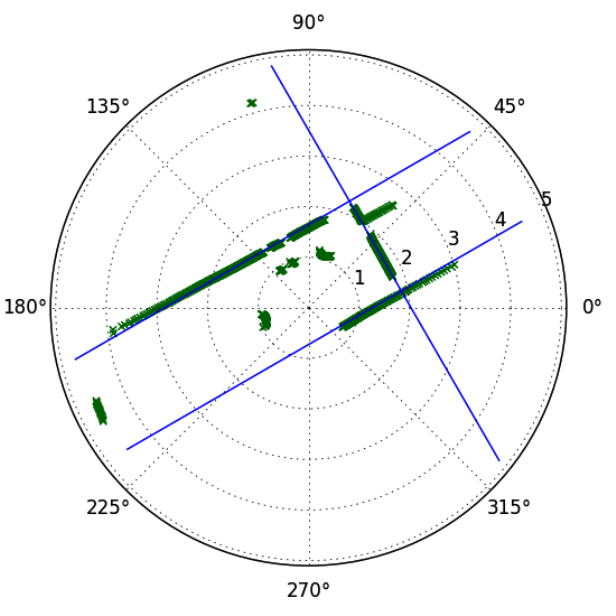
\includegraphics[width=\textwidth]{hough3}
 		 \caption{Detected lines}
      \end{subfigure}%
          \caption{Example 2 of Hough Transform being robust to people.}
          \label{fig: hough3}
  \end{figure}
 
\subsection{Measurement Model and the corresponding differentials}
\label{sec:linear_math}
Once the lines in the data are recovered, we need an effective representation to store them. The common, slope-point form has a major disadvantage when trying to represent perfectly vertical lines and the two point form will expand the size of the measurement vector $ z $ increasing the calculation required for \ekf. So it is preferable to represent it in the normal form where, just the coordinates of the point of intersection of the normal from the origin to the line is stored. For example, in Figure~\ref{fig: normal_form} the line can be represented solely by the point $ D $.

\begin{figure}
\centering
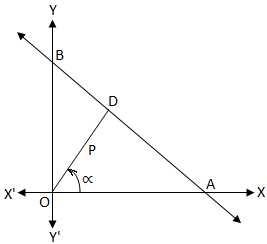
\includegraphics[width=0.45\textwidth]{normal_form}
\caption{Normal form of a line.}
\label{fig: normal_form}
\end{figure}

Once we have a line, we need to convert it to the inertial frame of reference as in section \ref{sec:Spike_math}. Unlike point features we are not trying to find the same point in a different frame but the same line. In Figure~\ref{fig: wall_to_world} we have point $ P_1 $ in robot frame and we need to find point $ P_2 $ in inertial given coordinates of the robot in inertial frame as $ P_r $. For which we use Algorithm \ref{alg: wall_to_world}.
\begin{figure}
\centering
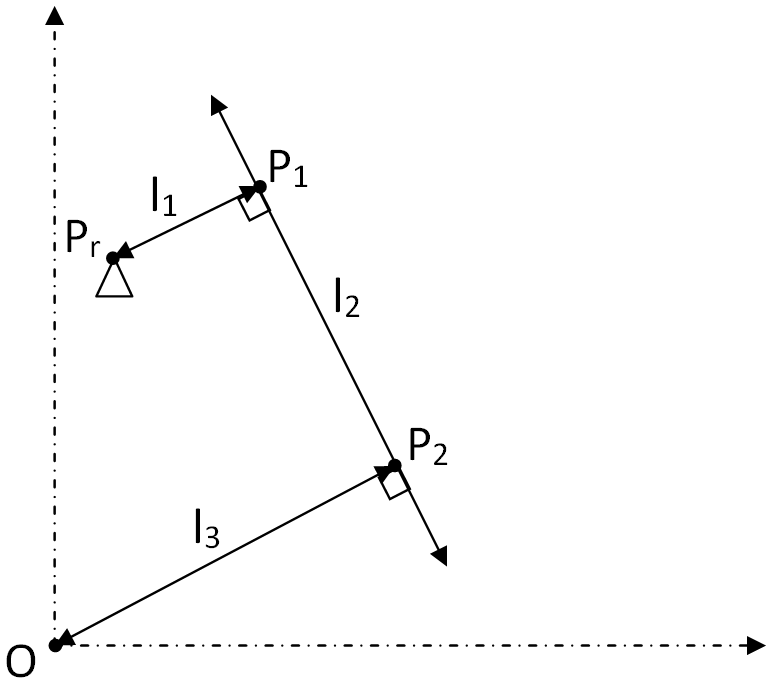
\includegraphics[width=0.45\textwidth]{wall_to_world}
\caption{Line in robot frame and world frame.}
\label{fig: wall_to_world}
\end{figure}

\begin{algorithm}[]
	\begin{enumerate}
		\item Convert point $ P_1 $ from robot frame of reference to inertial frame as in section \ref{sec:Spike_math}
		\item Given points $ P_r $ and $ P_1 $ in inertial frame, the Equation~of line $ l_1 $ is found using two point form of a line
		\item Since $ l1 \perp l2 $ the slope of $ l_2 $ is the negative reciprocal of the slope of $ l_1 $. 
		\item Using the slope and the point $ P_1 $ the Equation~of line $ l_2 $ is found using slope-point form of a line.
		\item The Equation~of line l3 is found similarly using slope of $ l_1 $ and point $ O $. 
		\item Solving equations for $ l_3 $ and $ l_2 $ we get the coordinates of point $ P_2 $. 
	\end{enumerate}
\caption{To convert linear features from robot frame to inertial frame.}
\label{alg: wall_to_world}
\end{algorithm}

Once we have the landmark in the world frame we need to see if it corresponds to any existing landmark in the map. We check this by comparing both the perpendicular distances between the walls and the angle between the walls. This allows us to have 2 tuning parameters so that the association can be weighted as desired. Usually since most walls in an indoor environments are at right angles, the variation allowed in angle for the association is larger compared to distance. 

Algorithm \ref{alg: wall_to_world} is also called the inverse measurement model as in subsequent time steps for the measurement model we do the exact opposite process. That is given a line using it's normal form in inertial frame, we need to get the \textit{measurement} from the robot. That is, we need the perpendicular distance from the robot to the wall and the angle of the laser beam which would hit the wall normally. For this given coordinate pf point $ P_2 $ as $ (x_2,y_2) $ and the robot pose as $ (x_r,y_r,\theta_r) $ we get $ P_1 $ using Equation~\ref{eq:lineModel1}. 

\begin{equation}
	\label{eq:lineModel1}
	x_1 = x_2 - \frac{y_2 ( x_2 y_ r- y_2 x_r)}{(x_2^2 + y_2^2)}
	\qquad
	y_1 = y_2 + \frac{x_2 ( x_2 y_ r- y_2 x_r)}{(x_2^2 + y_2^2)}
\end{equation}

\begin{equation}
	\label{eq:lineModel2}
	r=\sqrt{(y_1-y_r)^2+(x_1-x_r)^2}
	\qquad
	\alpha = \tan^{-1}\left(\frac{y_1-y_r}{x_1-x_r}\right)-\theta_r
\end{equation}

Once we have $ P_1 $, we can find the perpendicular distance $ r $ and angle $ \alpha $ using Equation~\ref{eq:lineModel2} giving measurement model $ h $ as per Equation~\ref{eq:lineModel3}. This measurement can be used to calculate the \textit{innovation} as per Equation~\ref{eq:EKF_8}. 

\begin{equation}
	\label{eq:lineModel3}
	h=\begin{bmatrix}
	r\\\alpha
	\end{bmatrix}
\end{equation}

For calculating the \textit{Kalman Gain}, we need the Jacobian matrix $ H $. As each wall is independent of the other, this has the same structure as explained in section \ref{sec:Spike_math} and is given by Equation~\ref{eq:SpikeMath3}. We derive each of the terms separately as per Equation~\ref{eq:lineModel5} and \ref{eq:lineModel6}.  

\begin{subequations}
\label{eq:lineModel5}
	\begin{align}
	\beta &= \frac{x_rx_1-x_1^2-y_1^2+y_ry_1}{x_1^2+y_1^2}\\
	\frac{\partial r}{\partial x_r} &= 2x_1\beta \quad
	\frac{\partial r}{\partial x_r} = 2y_1\beta \quad
	\frac{\partial r}{\partial \theta_r} = 0 \\
	\frac{\partial \alpha}{\partial x_r} &= 0 \quad 
	\frac{\partial \alpha}{\partial y_r} = 0 \quad 
	\frac{\partial \alpha}{\partial \theta_r} = -1
	\end{align}
\end{subequations}

\begin{subequations}
\label{eq:lineModel6}
	\begin{align}	
	\gamma &= \frac{x_rx_1-x_1^2-y_1^2+y_ry_1}{x_1^2+y_1^2} \\
	\frac{\partial r}{\partial x_1} &= 
	-2x_1\gamma^2 - 2\gamma(2x_1-x_r) \\
	\frac{\partial r}{\partial y_1} &= 
	-2y_1\gamma^2 - 2\gamma(2y_1-y_r)	\\
	\frac{\partial \alpha}{\partial x_1} &=  \frac{-y_1}{x_1^2+y_1^2}\qquad
	\frac{\partial \alpha}{\partial y_1} =
	\frac{x_1}{x_1^2+y_1^2} 
	\end{align}
\end{subequations}

Having the Jacobian matrices we can use the same observer error given by Equation~\ref{eq:SpikeMath5} to correct the position estimate using equations \ref{eq:EKF_7} to \ref{eq:EKF_9}.